% Created 2026-05-01 sex 01:09
% Intended LaTeX compiler: lualatex
\documentclass[12pt,a4paper]{article}
\usepackage{fgv-paper}
\geometry{a4paper,left=3cm,right=2cm,top=3cm,bottom=2cm,headheight=58pt,headsep=18pt,footskip=1.2cm}
\usepackage{float}
\usepackage{graphicx}
\usepackage{caption}
\usepackage{xcolor}
\usepackage{tikz}
\usepackage{fancyhdr}
\usepackage{tcolorbox}
\usepackage{tabularray}
\usepackage{booktabs}
\usepackage{tabularx}
\usepackage{array}
\usepackage{longtable}
\usepackage{ltablex}
\keepXColumns
\setlength{\emergencystretch}{3em}
\sloppy
\definecolor{FGVHeaderBlueDark}{HTML}{003B71}
\definecolor{FGVHeaderBlueMid}{HTML}{006BB6}
\definecolor{FGVHeaderBlueLight}{HTML}{8FD3F4}
\setlength{\headheight}{58pt}
\setlength{\headsep}{18pt}
\newcommand{\FGVHeaderLogoInclude}{\IfFileExists{fgv.png}{
\includegraphics[height=1.05cm]{fgv.png}}{}}
\newcommand{\FGVHeaderGradientRule}{\begin{tikzpicture}[baseline=(current bounding box.center)]\shade[left color=FGVHeaderBlueDark,middle color=FGVHeaderBlueMid,right color=FGVHeaderBlueLight] (0pt,0pt) rectangle (\headwidth,2pt);\end{tikzpicture}}
\newcommand{\FGVHeaderBlock}{\makebox[\headwidth][l]{\begin{minipage}[t]{\headwidth}\FGVHeaderLogoInclude\\[-1pt]\FGVHeaderGradientRule\end{minipage}}}
\fancypagestyle{fgvreportstyle}{%
\fancyhf{}%
\fancyhead[L]{\FGVHeaderBlock}%
\renewcommand{\headrulewidth}{0pt}%
\fancyfoot[C]{\thepage}%
}
\fancypagestyle{plain}{%
\fancyhf{}%
\fancyhead[L]{\FGVHeaderBlock}%
\renewcommand{\headrulewidth}{0pt}%
\fancyfoot[C]{\thepage}%
}
\AtBeginDocument{\pagestyle{fgvreportstyle}\thispagestyle{fgvreportstyle}}
\author{Gustavo M. Mendes de Tarso}
\date{29/04/2026}
\title{Atividade Aula 1}
\usepackage[backend=biber,style=apa]{biblatex}
\addbibresource{atividade_politicas_publicas_teorias_analises_aula_1_com_mapa.bib}

\begin{document}

\begingroup
\linespread{1}\selectfont
\begin{tcolorbox}[title=Ficha Técnica, colback=gray!5,colframe=gray!40,boxrule=0.4pt,sharp corners]
\begin{tblr}{rowsep=1pt,stretch=1, rows={t}, colspec={Q[l,2.8cm] X[l]}}
\textbf{Curso} & Mestrado Profissional em Gestão e Políticas Públicas \\
\textbf{Turma} & -- \\
\textbf{Pólo} & -- \\
\textbf{Disciplina} & Teorias da Administração Pública \\
\textbf{Professor} & -- \\
\textbf{Aluno(s)} & Gustavo M. Mendes de Tarso \\
\textbf{Data} & 29/04/2026 \\
\textbf{Título do trabalho} & Atividade Aula 1 \\
\end{tblr}
\end{tcolorbox}
\endgroup
\clearpage
\section{Introdução}
\label{sec:org6f56491}
A análise de políticas públicas dispõe de diferentes modelos teóricos para explicar por que determinados problemas alcançam a agenda governamental, como alternativas são selecionadas e de que modo atores organizados disputam interpretações e soluções ao longo do tempo. No conjunto de textos mobilizados nesta atividade, duas abordagens ocupam posição central: o modelo de múltiplos fluxos e o modelo das coalizões de defesa. Ambos integram o repertório contemporâneo da área, mas partem de pressupostos distintos sobre a dinâmica do processo decisório, o papel das ideias, a organização dos atores e o ritmo das mudanças institucionais \autocites{capella2022multiplos}{araujoSilva2022coalizoes}.
Com base exclusivamente no corpus local disponibilizado, este trabalho examina os capítulos teóricos sobre o modelo de múltiplos fluxos e sobre o modelo das coalizões de defesa, bem como dois artigos empíricos formalmente selecionados para a atividade: o estudo de \textcite{bijos2024ifi} sobre a criação da Instituição Fiscal Independente brasileira e o artigo de \textcite{ferreira2019habitacional} sobre a política habitacional no Brasil a partir do Advocacy Coalition Framework. O objetivo é apresentar uma leitura analítica e comparativa dos textos, destacando suas contribuições para a compreensão do tema da aula: as teorias que explicam por que o governo passa a deliberar sobre determinados problemas e como diferentes arranjos explicativos ajudam a interpretar processos concretos de política pública.
Do ponto de vista metodológico, a atividade parte da leitura substantiva de todos os textos disponíveis no cache local. Os capítulos do livro fornecem a base conceitual e interpretativa da discussão, enquanto os artigos selecionados permitem observar a operacionalização empírica das teorias em casos brasileiros. Essa combinação é particularmente produtiva porque aproxima formulação teórica e análise aplicada. Ao mesmo tempo, é preciso reconhecer uma limitação do corpus: o arquivo do livro contém vários capítulos, mas as orientações da atividade destacam especialmente os capítulos sobre múltiplos fluxos e coalizões de defesa; assim, a análise concentra-se nesses conteúdos identificados com segurança no material fornecido, evitando extrapolações indevidas sobre capítulos não explorados em detalhe pelo conjunto de instruções e metadados disponíveis.
\section{Resumo individual dos textos}
\label{sec:org1407e4d}
\subsection{O modelo de múltiplos fluxos}
\label{sec:orgb2fa5d7}
O capítulo de \textcite{capella2022multiplos} apresenta o modelo de múltiplos fluxos como uma das explicações mais influentes para compreender a formação da agenda governamental em contextos de ambiguidade, informação imperfeita e racionalidade limitada. O argumento central é que políticas públicas não emergem de um processo linear em que problemas identificados conduzem automaticamente a soluções. Ao contrário, a agenda resulta do acoplamento contingente entre três fluxos relativamente independentes: o fluxo dos problemas, o fluxo das alternativas e o fluxo da política \autocites{capella2022multiplos}{kingdon2003agendas}.
O objetivo do texto é duplo. Em primeiro lugar, reconstruir os fundamentos do modelo proposto por Kingdon, ressaltando sua ruptura com interpretações excessivamente racionalistas do processo de formulação de políticas. Em segundo lugar, discutir a difusão do modelo no campo da análise de políticas públicas e sua utilidade para investigações empíricas. A autora enfatiza que a agenda não é um simples espelho das necessidades sociais, mas o resultado de processos seletivos nos quais apenas alguns temas são definidos como merecedores de atenção governamental \autocite{capella2022multiplos}.
No fluxo dos problemas, o texto mostra que condições sociais não se convertem automaticamente em problemas públicos. Para isso, são necessários mecanismos de interpretação e reconhecimento, como indicadores, eventos focais e feedbacks de políticas anteriores. O problema, portanto, é construído politicamente. Já no fluxo das alternativas, a autora destaca o papel das comunidades de especialistas, que elaboram propostas e disputam sua viabilidade técnica e política. Nem toda alternativa sobrevive; apenas aquelas que conseguem certa aceitabilidade, consistência e capacidade de difusão permanecem disponíveis para eventual adoção. No fluxo da política, por sua vez, entram em cena fatores como humor nacional, mudanças governamentais, correlação de forças e pressões organizadas, elementos que afetam a receptividade do sistema político a determinadas pautas \autocite{capella2022multiplos}.
Um conceito decisivo do capítulo é o de “janela de oportunidade”, entendido como o momento em que os fluxos podem ser articulados de forma favorável. Nessas conjunturas, empreendedores de políticas atuam para acoplar problema, solução e ambiente político. Essa figura do empreendedor é relevante porque permite compreender a agência estratégica sem supor controle total sobre o processo. O ator não cria livremente as condições; ele explora oportunidades abertas por conjunturas específicas \autocites{capella2022multiplos}{kingdon2003agendas}.
A estrutura argumentativa do texto é didática e cumulativa. Parte-se dos pressupostos gerais do modelo, detalham-se os três fluxos, explicam-se os mecanismos de acoplamento e, por fim, indicam-se as potencialidades analíticas da abordagem. A contribuição do capítulo para o tema da aula é direta: ele oferece uma resposta consistente à pergunta sobre por que o governo decide deliberar sobre certos assuntos. A resposta não reside em uma causalidade única, mas na convergência circunstancial de dinâmicas distintas, mediada por atores e oportunidades.
Em termos críticos, o capítulo também sugere que o modelo é mais forte para explicar entrada na agenda do que para interpretar fases posteriores de implementação ou mudança institucional prolongada. Além disso, a ênfase em contingência e acoplamento pode dificultar a especificação de causalidades mais estáveis. Ainda assim, sua relevância é inequívoca para situações em que a abertura da agenda depende de conjunturas fluidas, redefinições de problemas e empreendedorismo político \autocite{capella2022multiplos}.
\subsection{O modelo das coalizões de defesa}
\label{sec:org0210909}
O capítulo de \textcite{araujoSilva2022coalizoes} apresenta o modelo das coalizões de defesa como uma teoria voltada a explicar processos de mudança e estabilidade em subsistemas de políticas públicas ao longo de períodos mais extensos. Diferentemente do foco mais concentrado do modelo de múltiplos fluxos sobre agenda e decisão, o Advocacy Coalition Framework parte da ideia de que atores de diferentes organizações se agregam em torno de sistemas compartilhados de crenças e, a partir deles, disputam a orientação das políticas no interior de um subsistema \autocites{araujoSilva2022coalizoes}{sabatier1999theories}.
O texto enfatiza que políticas públicas são arenas de conflito interpretativo. Nesse sentido, as coalizões de defesa não são meras alianças circunstanciais; elas se estruturam por afinidades normativas e cognitivas, especialmente em torno de crenças profundas, crenças centrais de política e aspectos secundários. Tal distinção é importante porque permite compreender por que certas posições se mostram mais resistentes à mudança do que outras. Mudanças em aspectos secundários são relativamente frequentes, enquanto alterações nas crenças centrais exigem pressões mais intensas, geralmente associadas a choques externos, mudanças socioeconômicas ou reconfigurações do subsistema \autocite{araujoSilva2022coalizoes}.
O objetivo do capítulo é introduzir os fundamentos do modelo, explicar seus principais componentes analíticos e indicar sua aplicabilidade ao estudo de políticas públicas. Entre esses componentes, destacam-se o subsistema de política, as coalizões de defesa, os recursos mobilizados pelos atores, o papel dos brokers de política e os mecanismos de aprendizado orientado à política. Este último aspecto é central, pois o modelo não reduz o processo a mera disputa de poder: ele reconhece que evidências, informações e experiências podem produzir ajustamentos, ainda que tais mudanças sejam filtradas por crenças previamente estabelecidas \autocite{araujoSilva2022coalizoes}.
A argumentação do capítulo mostra que o modelo é especialmente adequado para contextos em que múltiplos atores — governamentais e não governamentais — interagem de forma continuada ao redor de uma política setorial. Nesse tipo de situação, a análise de episódios isolados não basta; é preciso observar trajetórias, disputas de longo prazo, institucionalização de fóruns e efeitos de eventos externos. Com isso, a abordagem amplia a compreensão do processo político para além do momento inicial da agenda, incorporando a persistência dos conflitos e o papel das crenças na orientação da ação coletiva \autocite{araujoSilva2022coalizoes}.
Para o tema da aula, o capítulo contribui ao demonstrar que a deliberação governamental sobre uma questão não decorre apenas de sua entrada na agenda, mas também da capacidade de coalizões organizadas manterem, alterarem ou deslocarem os sentidos da política ao longo do tempo. Em outras palavras, o governo passa a deliberar sobre um tema, mas o conteúdo dessa deliberação depende da estrutura do subsistema, dos recursos dos atores e da disputa entre visões concorrentes.
Como limite, o próprio emprego do modelo exige um volume robusto de informação empírica sobre atores, crenças, instituições e séries temporais, o que pode tornar sua operacionalização complexa. Ainda assim, trata-se de um instrumental poderoso para explicar conflitos duradouros, mudanças graduais e choques de trajetória em políticas públicas \autocites{araujoSilva2022coalizoes}{sabatier1999theories}.
\subsection{O nascimento da Instituição Fiscal Independente brasileira: explicação à luz do modelo de Kingdon}
\label{sec:org15ebecc}
O artigo de \textcite{bijos2024ifi} aplica o modelo de Kingdon ao caso da criação da Instituição Fiscal Independente (IFI) brasileira no âmbito do Senado Federal, em 2016. O problema de pesquisa consiste em explicar por que a IFI foi criada naquele momento, tendo em vista que propostas semelhantes já circulavam anteriormente sem lograr institucionalização. O estudo é particularmente relevante porque transforma uma teoria sobre agenda e formulação em instrumento de leitura de um caso concreto da política fiscal brasileira.
O autor sustenta que a criação da IFI pode ser entendida como resultado do acoplamento dos três fluxos do modelo de múltiplos fluxos. No fluxo dos problemas, a crise fiscal, a deterioração das contas públicas e a desconfiança em relação às informações produzidas pelo Executivo criaram um ambiente favorável ao reconhecimento de um problema público ligado ao monitoramento independente da política fiscal \autocite{bijos2024ifi}. O tema não se reduzia à existência de dificuldades econômicas, mas à percepção de insuficiência dos mecanismos institucionais de controle e transparência.
No fluxo das alternativas, o artigo mostra que a ideia de uma instituição fiscal independente já era conhecida no debate especializado e possuía referência em experiências internacionais. Assim, quando a janela de oportunidade se abriu, havia uma solução disponível e intelectualmente legitimada. Esse elemento é fundamental no modelo de Kingdon: problemas não geram automaticamente soluções; é preciso que alternativas estejam amadurecidas e circulem em comunidades de especialistas e formuladores \autocites{bijos2024ifi}{kingdon2003agendas}.
No fluxo da política, o estudo identifica as condições que tornaram politicamente viável a criação da IFI: o contexto pós-crise, a reconfiguração do cenário político em torno da responsabilização fiscal, a atuação do Senado e a presença de atores dispostos a patrocinar a proposta. O autor destaca o papel do empreendedor de políticas, figura que articula os fluxos e aproveita a janela de oportunidade para impulsionar a mudança institucional. Nessa chave, a criação da IFI não aparece como simples consequência técnica da crise fiscal, mas como produto de uma conjuntura política específica, interpretada e explorada por atores estratégicos \autocite{bijos2024ifi}.
Metodologicamente, o artigo é consistente ao articular reconstrução histórica do processo decisório com categorias analíticas claramente derivadas do modelo teórico. A explicação é organizada de maneira a evidenciar como cada fluxo contribuiu para o desfecho observado. Essa estrutura fortalece o argumento porque evita o uso apenas retórico da teoria; ao contrário, o modelo orienta a interpretação do caso.
A principal contribuição do texto para a atividade é mostrar a potência do modelo de múltiplos fluxos em contextos de mudança institucional relativamente concentrada, marcados por crises, oportunidade política e disponibilidade de alternativas. O artigo demonstra que a agenda governamental pode ser compreendida como uma arena em que ideias preexistentes ganham tração apenas quando problemas são socialmente reconhecidos e o ambiente político se torna receptivo.
Um ponto crítico, contudo, é que a própria força do modelo está vinculada ao recorte do problema. O artigo explica muito bem a emergência institucional da IFI, mas não se dedica prioritariamente a examinar, em igual profundidade, os efeitos posteriores da instituição no subsistema fiscal. Isso não é propriamente uma falha, mas uma delimitação coerente com a teoria mobilizada. Assim, o estudo confirma a adequação do modelo de Kingdon para a explicação do momento de surgimento de uma política ou instituição \autocite{bijos2024ifi}.
\subsection{Política habitacional no Brasil: uma análise das coalizões de defesa do Sistema Nacional de Habitação de Interesse Social versus o Programa Minha Casa, Minha Vida}
\label{sec:orgc0747d3}
O artigo de \textcite{ferreira2019habitacional} examina a política habitacional brasileira entre 1992 e 2014 a partir do modelo das coalizões de defesa. O foco recai sobre a tensão entre o Sistema Nacional de Habitação de Interesse Social (SNHIS) e o Programa Minha Casa, Minha Vida (PMCMV), permitindo analisar como diferentes conjuntos de atores, valores e estratégias disputaram os rumos da política no período. Trata-se de um caso empiricamente rico para o Advocacy Coalition Framework, pois envolve longa duração, múltiplos atores e conflitos interpretativos sobre instrumentos, prioridades e desenho institucional.
O objetivo central do estudo é compreender as mudanças institucionais ocorridas na política habitacional, identificando as crenças e coalizões presentes tanto na formulação do SNHIS quanto na posterior ascensão do PMCMV. Para isso, os autores recorrem a um conjunto diverso de fontes — legislação, normas, atas, registros de conferências e entrevistas —, o que reforça o caráter substantivo da análise \autocite{ferreira2019habitacional}.
O artigo argumenta que o SNHIS expressava uma coalizão orientada por participação social, planejamento federativo, institucionalização de fundos e construção de uma política habitacional mais integrada. Sua tramitação lenta e longa no Congresso revelaria, por um lado, a complexidade de consolidar esse projeto e, por outro, a densidade do arranjo participativo que o sustentava. Em contraste, o PMCMV emergiu em contexto de crise econômica e foi aprovado com rapidez, priorizando uma lógica de estímulo econômico, escala de produção e resposta célere, ainda que com menor centralidade dos mecanismos participativos que haviam caracterizado o SNHIS \autocite{ferreira2019habitacional}.
A análise das coalizões permite mostrar que a mudança não se explica apenas por decisão governamental pontual, mas por disputa entre crenças e prioridades distintas no interior do subsistema habitacional. Uma coalizão valorizava a habitação de interesse social em moldes mais participativos e articulados; outra operava com maior ênfase em dinamização econômica, produção habitacional em larga escala e capacidade executiva. Essa oposição evidencia a utilidade do Advocacy Coalition Framework para captar não apenas a alternância de instrumentos, mas a reorientação do sentido da política pública \autocites{ferreira2019habitacional}{araujoSilva2022coalizoes}.
O texto também é relevante por demonstrar que mudanças institucionais podem ocorrer sem completa substituição de um arranjo pelo outro. Há sobreposições, tensões e deslocamentos que produzem reconfigurações do subsistema. Nessa perspectiva, o PMCMV não aparece apenas como um programa adicional, mas como uma alternativa que reorganiza prioridades e altera o equilíbrio entre coalizões.
A contribuição do artigo para a atividade é expressiva porque ele exemplifica, em caso brasileiro, como o modelo das coalizões de defesa ajuda a compreender processos duradouros e disputas em torno da orientação de uma política setorial. Seu limite, em termos analíticos, decorre menos do trabalho em si do que da própria exigência do modelo: a explicação é densa e dependente de detalhamento institucional e histórico, o que torna a leitura mais complexa do que abordagens centradas em episódios decisórios específicos. Ainda assim, o artigo mostra de forma convincente que políticas públicas são arenas de conflito entre projetos, e que a deliberação governamental se enraíza em disputas ideacionais e organizacionais persistentes \autocite{ferreira2019habitacional}.
\section{Comparação entre os textos}
\label{sec:org6b74389}
Os textos do corpus se articulam em torno de uma questão comum: como explicar a emergência, a transformação e a disputa em torno das políticas públicas. Contudo, eles operam em níveis analíticos diferentes. Os capítulos teóricos oferecem a arquitetura conceitual dos modelos, enquanto os artigos empíricos demonstram sua aplicação em casos brasileiros. Essa combinação permite observar a complementaridade entre teoria e empiria de modo particularmente claro.
A principal convergência entre o capítulo sobre múltiplos fluxos e o capítulo sobre coalizões de defesa está na recusa de explicações estritamente lineares e racionalistas do processo de políticas públicas. Em ambos, ideias, interpretações e disputas simbólicas importam. O processo decisório não é tratado como simples resposta técnica a problemas objetivos. Tanto \textcite{capella2022multiplos} quanto \textcite{araujoSilva2022coalizoes} atribuem centralidade à construção social dos problemas, à competição entre atores e à relevância de arranjos institucionais na filtragem das decisões.
Apesar dessa convergência geral, as divergências entre os modelos são substantivas. O modelo de múltiplos fluxos privilegia a dinâmica da agenda, a contingência e o acoplamento entre fluxos relativamente autônomos. Já o modelo das coalizões de defesa enfatiza a estabilidade e a mudança em subsistemas de políticas no longo prazo, estruturadas por crenças compartilhadas e disputas entre coalizões \autocites{capella2022multiplos}{araujoSilva2022coalizoes}. Em termos simplificados, Kingdon ajuda a explicar por que uma questão entra na agenda em determinado momento; Sabatier ajuda a compreender como visões concorrentes sustentam ou transformam políticas ao longo do tempo.
Os artigos empíricos reforçam essa distinção. O estudo de \textcite{bijos2024ifi} é exemplar de uma situação em que a abertura de oportunidade política, somada à disponibilidade de solução e ao reconhecimento de um problema, explica a criação de uma nova instituição. Trata-se de um caso compatível com o foco de Kingdon em agenda e decisão. Já o artigo de \textcite{ferreira2019habitacional} examina um processo mais prolongado, no qual diferentes coalizões disputam os rumos da política habitacional e reorientam seus instrumentos e instituições. Aqui, a lente das coalizões de defesa mostra-se mais adequada.
Há também diferenças metodológicas relevantes. O artigo sobre a IFI reconstrói uma conjuntura decisória e identifica o acoplamento entre fluxos, enfatizando a janela de oportunidade. O estudo sobre habitação, por sua vez, requer um mapeamento mais amplo de atores, crenças, instituições e documentos ao longo de mais de duas décadas. Isso indica que a escolha da teoria não é apenas conceitual, mas também metodológica: diferentes modelos orientam diferentes estratégias de investigação.
Um ponto adicional de comparação é a forma como os textos tratam a agência. Em Kingdon, ela aparece sobretudo na figura do empreendedor de políticas, ator capaz de acoplar fluxos em momentos oportunos \autocites{kingdon2003agendas}{capella2022multiplos}. No Advocacy Coalition Framework, a agência é mais distribuída entre coalizões, brokers e organizações que operam no subsistema \autocites{araujoSilva2022coalizoes}{sabatier1999theories}. Assim, enquanto um modelo destaca a atuação estratégica em conjunturas críticas, o outro realça a ação coletiva e continuada em arenas institucionalizadas.
Os textos, portanto, não são rivais absolutos, mas instrumentos analíticos com ênfases distintas. Lidos em conjunto, eles mostram que o estudo das políticas públicas exige atenção simultânea aos momentos de abertura da agenda e às disputas prolongadas que dão conteúdo, direção e permanência às decisões governamentais.
\section{Síntese analítica}
\label{sec:orgd479daa}
A leitura conjunta do corpus permite sustentar que a pergunta sobre por que o governo decide deliberar sobre uma determinada questão não admite resposta única. Os textos indicam, em vez disso, que a deliberação governamental decorre da interação entre construção de problemas, disponibilidade de alternativas, conjunturas políticas, organização de atores e disputas entre crenças. Em síntese, políticas públicas não nascem nem mudam apenas porque “há um problema”, mas porque esse problema é interpretado, disputado e articulado a soluções e interesses institucionalmente viáveis.
Sob essa perspectiva, o modelo de múltiplos fluxos oferece uma explicação especialmente forte para os momentos de emergência da agenda. Ele demonstra que a decisão de deliberar depende de uma convergência rara entre reconhecimento do problema, existência de alternativas e receptividade política. A análise de \textcite{bijos2024ifi} torna isso particularmente evidente: a IFI não foi criada apenas porque a crise fiscal existia, mas porque a crise ganhou visibilidade como problema institucional, havia uma solução disponível e atores souberam aproveitá-la em uma janela de oportunidade \autocites{bijos2024ifi}{capella2022multiplos}.
Já o modelo das coalizões de defesa é mais apropriado para compreender políticas que se desenvolvem em arenas estáveis de conflito e negociação ao longo do tempo. No caso da política habitacional, a oposição entre SNHIS e PMCMV não pode ser reduzida a uma escolha episódica de governo; ela expressa embates entre projetos, crenças e arranjos institucionais distintos. O artigo de \textcite{ferreira2019habitacional} evidencia que a deliberação governamental, nesse contexto, precisa ser lida como resultado de relações de força dentro de um subsistema, e não apenas como resposta a uma conjuntura momentânea \autocites{ferreira2019habitacional}{araujoSilva2022coalizoes}.
Uma compreensão mais ampla do tema da aula, portanto, emerge justamente da combinação entre os dois modelos. Kingdon ajuda a explicar \emph{quando} e \emph{como} uma questão alcança prioridade decisória. O Advocacy Coalition Framework ajuda a explicar \emph{quem} disputa seus significados e \emph{por que} determinadas orientações persistem ou são alteradas ao longo do tempo. Essa complementaridade é um dos principais ganhos analíticos do corpus.
Também se destaca, nos textos, a centralidade das ideias. Em ambos os modelos, as políticas públicas são atravessadas por interpretações concorrentes da realidade. Problemas não são dados brutos; são enquadrados. Soluções não são neutras; carregam pressupostos. Coalizões não se organizam apenas por interesse material imediato; também se estruturam em torno de crenças. Isso confere densidade política e cognitiva ao processo decisório, afastando leituras simplificadoras.
Ao mesmo tempo, os textos sugerem prudência analítica. Nenhum modelo explica tudo. O de múltiplos fluxos pode ser menos preciso para examinar disputas prolongadas em subsistemas complexos. O de coalizões de defesa exige uma base empírica extensa e pode ser menos econômico para explicar eventos decisórios concentrados. Reconhecer esses limites não reduz sua utilidade; ao contrário, melhora sua aplicação. A escolha do referencial teórico deve guardar relação com o tipo de problema investigado.
\section{Considerações finais}
\label{sec:orgcfc4d88}
Esta atividade mostrou que o estudo das políticas públicas exige atenção às diferentes temporalidades do processo decisório. Com base nos textos do corpus local, foi possível observar que a entrada de temas na agenda governamental e a disputa por seus significados são dimensões analiticamente relacionadas, mas não idênticas. O modelo de múltiplos fluxos, apresentado por \textcite{capella2022multiplos} e aplicado empiricamente por \textcite{bijos2024ifi}, é particularmente útil para compreender conjunturas em que problemas, alternativas e condições políticas convergem para produzir decisão. O modelo das coalizões de defesa, exposto por \textcite{araujoSilva2022coalizoes} e operacionalizado por \textcite{ferreira2019habitacional}, mostra-se mais adequado para interpretar conflitos duradouros em subsistemas de política e mudanças institucionais de maior extensão temporal.
A principal aprendizagem extraída do conjunto dos textos é que a deliberação governamental não pode ser explicada por determinismo técnico, nem por vontade política isolada. Ela depende de processos de construção social dos problemas, de disponibilidade de soluções legitimadas, de janelas de oportunidade, de coalizões organizadas e de disputas entre crenças e projetos. Assim, o tema da aula — por que o governo decide deliberar sobre determinada questão — revela-se menos como problema de escolha simples e mais como problema de articulação entre estruturas, ideias e agência.
Por fim, os casos brasileiros analisados reforçam a utilidade das teorias estudadas para além de sua formulação original. Tanto a criação da IFI quanto as mudanças na política habitacional demonstram que modelos teóricos de análise de políticas públicas podem iluminar processos concretos, desde que aplicados com rigor conceitual e sensibilidade ao contexto. A leitura integrada do corpus, portanto, não apenas resume textos, mas também oferece uma compreensão analítica consistente sobre os mecanismos pelos quais temas entram na agenda, são disputados e se institucionalizam no Estado brasileiro.

\printbibliography

\clearpage
\begingroup
\centering
{\Large\bfseries Mapa mental dos textos analisados\par}
\vspace{1em}
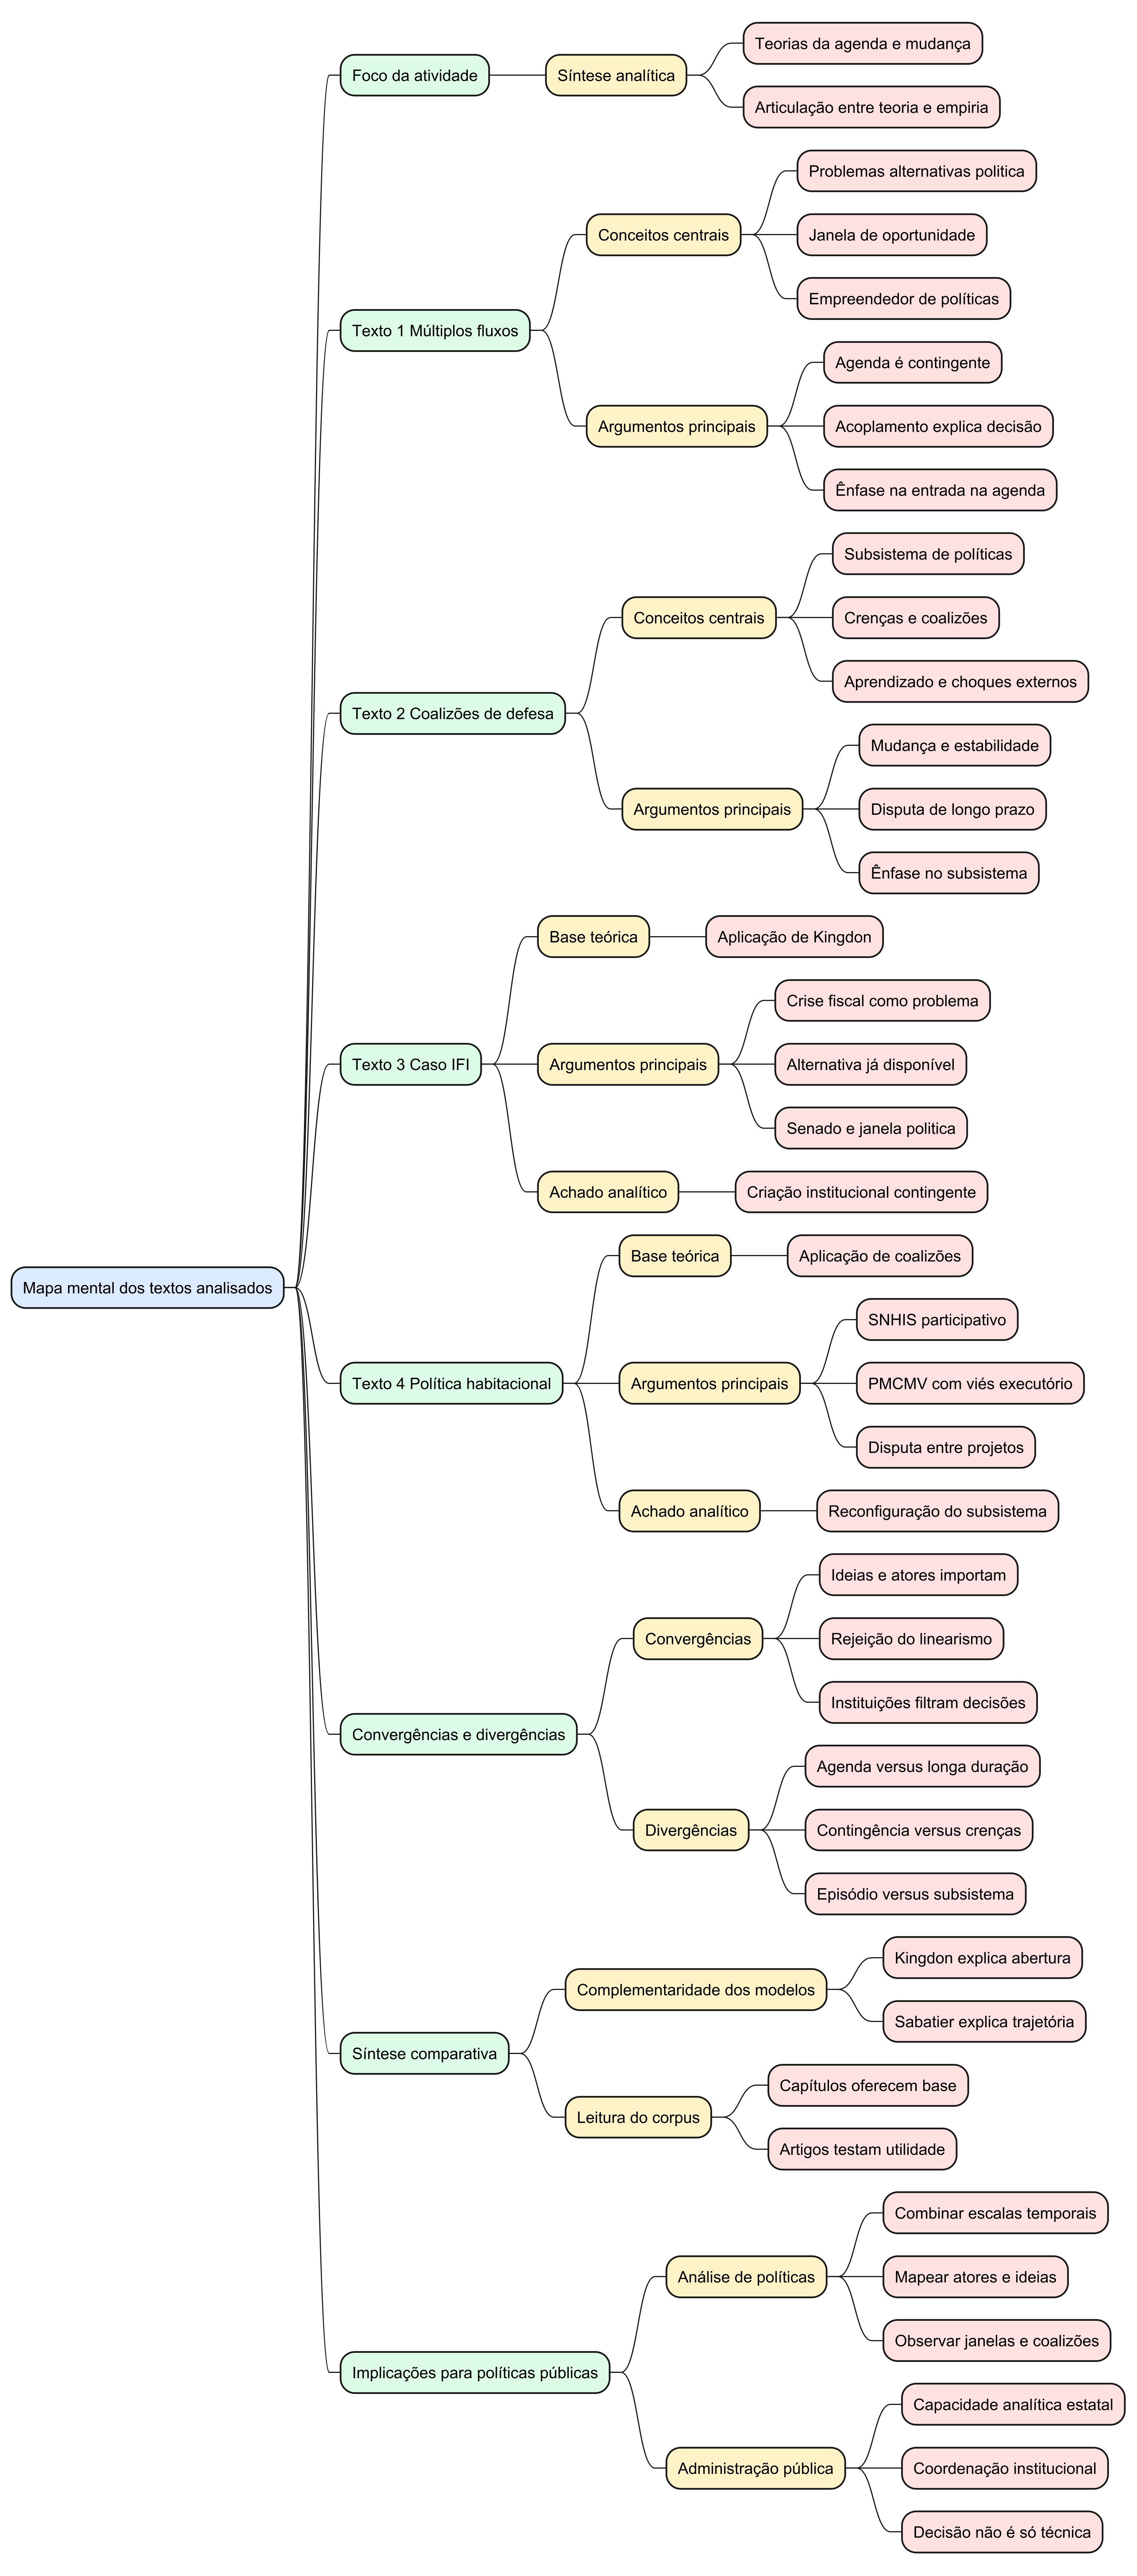
\includegraphics[width=\textwidth,height=0.86\textheight,keepaspectratio]{images/mapa_mental.png}
\par
\endgroup
\clearpage
\end{document}
